\subsection{Функциональная структура компилятора}
\label{impl:compiler} % \index{Chapter7}

Используя знания о MLIR и DaVinci, полученные в результате исследовательской
работы, приступим к описанию структуры компилятора. Он содержит новые диалекты,
которые на разных уровнях абстракции отражают особенности архитектуры DaVinci.
Перечислим их и отметим основные особенности:

\begin{enumerate}
    \item \textit{ascend} --- диалект крупноблочных операций. Является аналогом
          HLO, но операции в нём предъявляют требования к типам данных: матрицы
          должны быть расположены в блочном формате. Поэтому в процессе трансляции
          из HLO в ascend для входных и выходных данных вставляются операции
          фрактализации, т.е. приведения матрицы к нужному виду. Для остальных
          диалектов требование на формат данных сохраняется, при этом считается,
          что оно выполняется благодаря корректности представления графа
          исполнения в диалекте ascend.

    \item \textit{cce} --- диалект операций, схожих с ассемблерными инструкциями.
          Основная его особеннность заключается в сохранении семантики
          многомерных массивов, что позволяет упрощать процесс генерации таких
          операций и их верификации (проверки корректности).

    \item \textit{hivm} --- диалект непосредственных ассемблерных инструкций. Он в
          точности повторяет их семантику, что упрощает его трансляцию в llvm.
\end{enumerate}

Конвейер компиляции для девайса выглядит следующим образом:

\begin{figure}[h!]
      \centering
      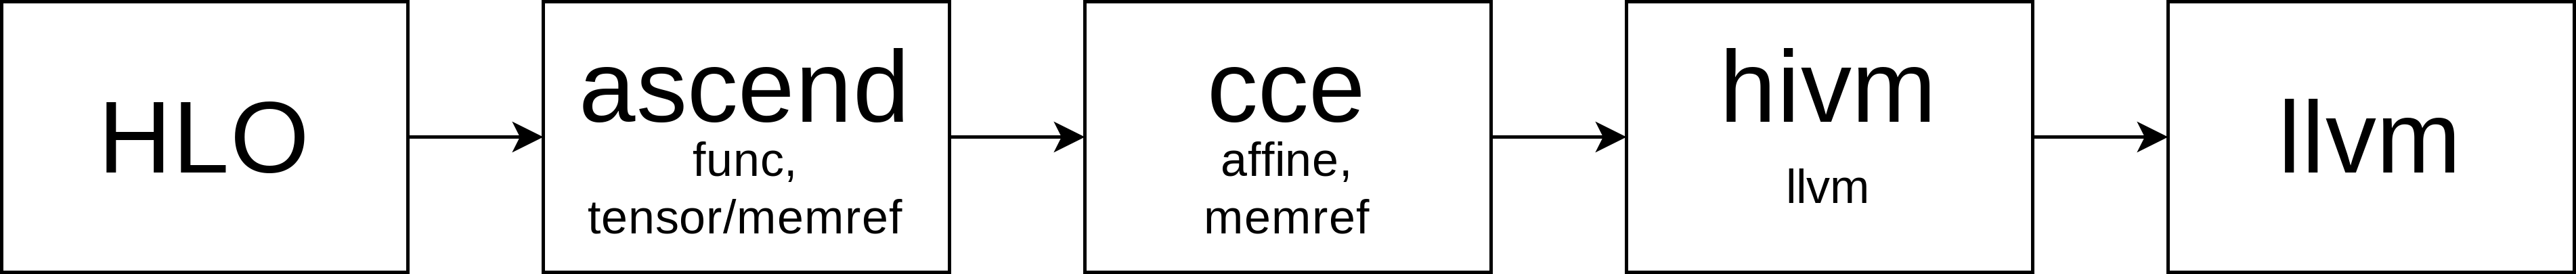
\includegraphics[scale=0.1]{Compiler.png}
      \caption{Конвейер компиляции для девайса}
  \end{figure}

В данной работе рассматривается трансляция от диалекта ascend к диалекту cce,
что соответствует переходу от крупноблочных операторов к операторам, схожих с
инструкциями процессора Ascend.
